\subsubsection{Model architecture}
\label{sub:comb_model_architecture}

\structure{General architecture ideas \& requirements}

\begin{figure}[h]
\begin{subfigure}{.5\textwidth}
  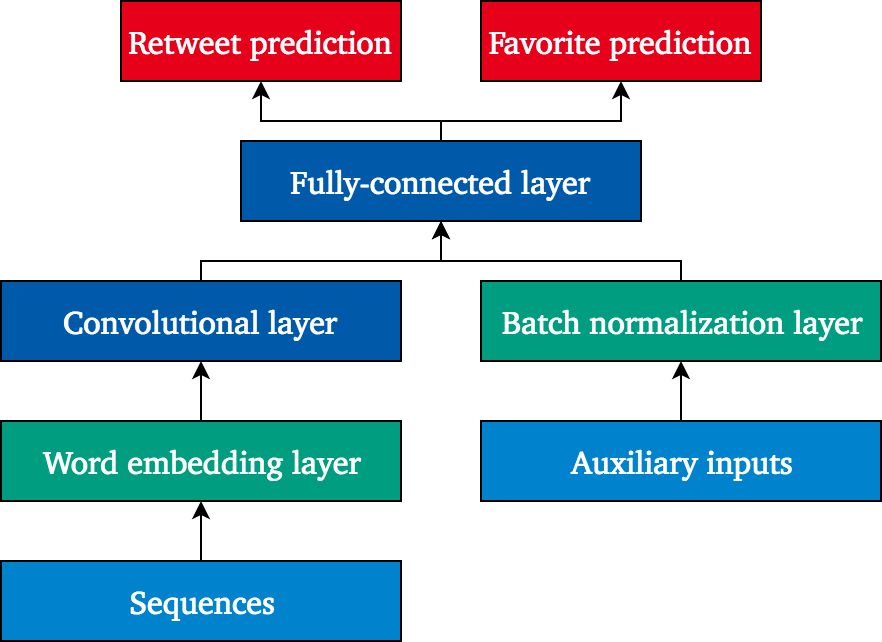
\includegraphics[width=.95\linewidth]{img/dm2_cnn}
  \caption{DM2-CNN}
  \label{fig:dm2_cnn}
\end{subfigure}%
\begin{subfigure}{.5\textwidth}
  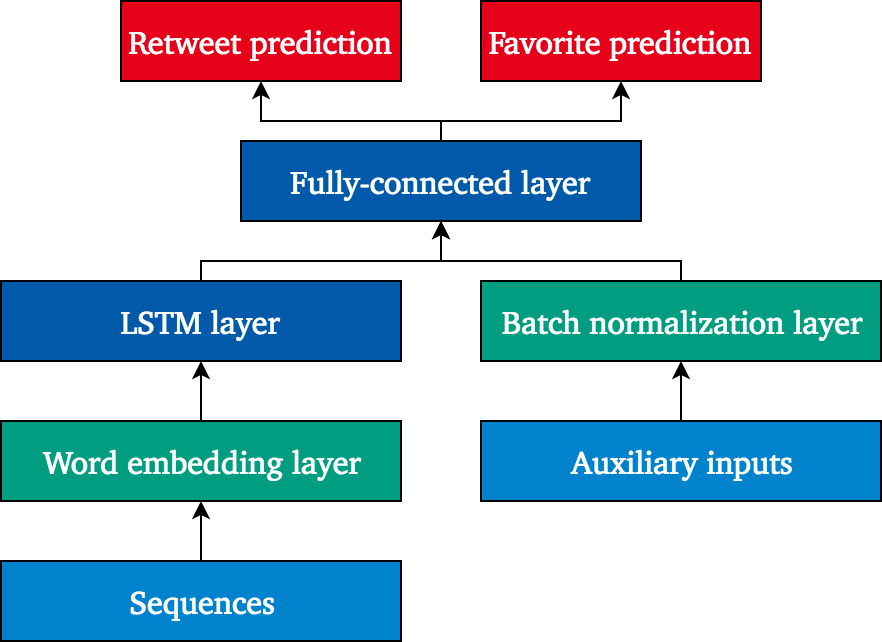
\includegraphics[width=.95\linewidth]{img/dm2_lstm}
  \caption{DM2-LSTM}
  \label{fig:dm2_lstm}
\end{subfigure}
\begin{subfigure}{.7\textwidth}
  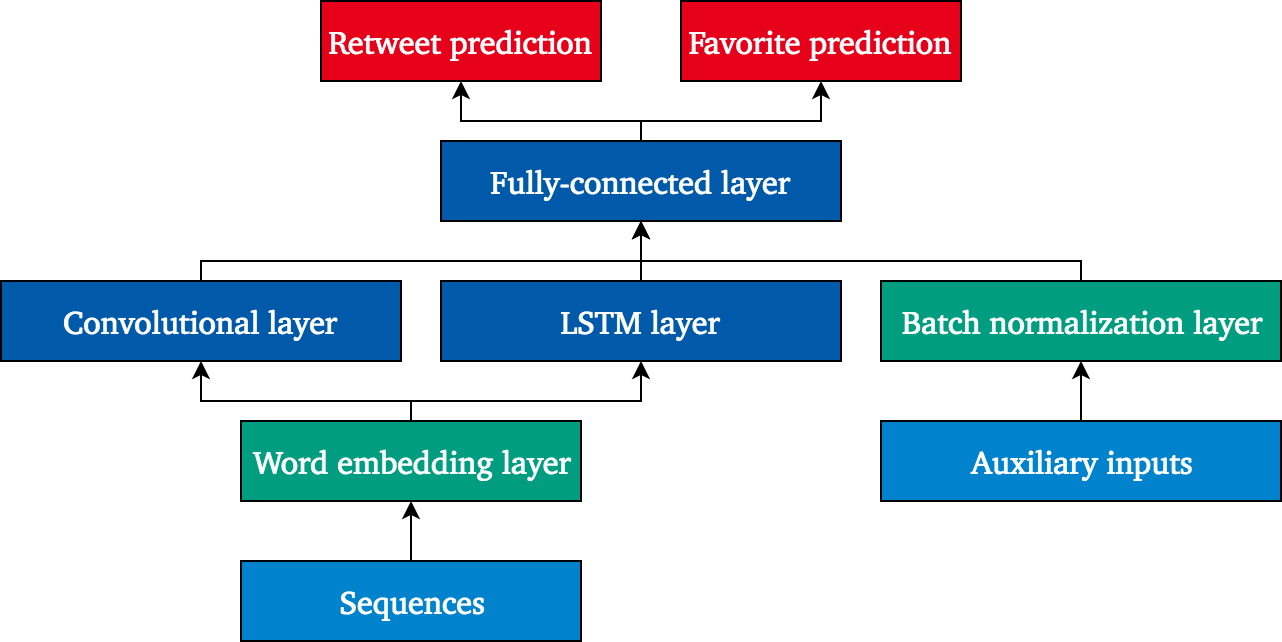
\includegraphics[width=.95\linewidth]{img/dm2_cnn_lstm}
  \caption{DM2-CNN-LSTM}
  \label{fig:dm2_cnn_lstm}
\end{subfigure}
\caption{Subset of evaluated architectures for multi-input models}
\label{fig:dm2_architectures}
\end{figure}

\structure{Model selection process}

\begin{table}
\begin{tabular}{llrr}
\toprule
Model architecture & Data set & Classification loss & Regression loss \\
\midrule
DM2-CNN & Combined & 0.7897 & \textbf{401.5174} \\
DM2-LSTM & Combined & 0.7628 & 411.2176 \\
DM2-CNN-LSTM & Combined & \textbf{0.7556} & 410.8704 \\
DM2-CNN2 & Combined & 0.7641 & 409.1842 \\
DM2-CNN3 & Combined & 0.8050 & 404.9901 \\
\bottomrule
\end{tabular}
\caption{Summary of multi-input model selection}
\label{tab:dm2_selection_results}
\end{table}
